%
% ---------------------------------------------------------------
% Copyright (C) 2012-2018 Gang Li
% ---------------------------------------------------------------
%
% This work is the default powerdot-tuliplab style test file and may be
% distributed and/or modified under the conditions of the LaTeX Project Public
% License, either version 1.3 of this license or (at your option) any later
% version. The latest version of this license is in
% http://www.latex-project.org/lppl.txt and version 1.3 or later is part of all
% distributions of LaTeX version 2003/12/01 or later.
%
% This work has the LPPL maintenance status "maintained".
%
% This Current Maintainer of this work is Gang Li.
%
%

\documentclass[
 size=14pt,
 paper=smartboard,  %a4paper, smartboard, screen
 mode=present, 		%present, handout, print
 display=slides, 	% slidesnotes, notes, slides
 style=tuliplab,  	% TULIP Lab style
 pauseslide,
 fleqn,leqno]{powerdot}

\usepackage{graphicx}
\usepackage{cancel}
\usepackage{caption}
\usepackage{stackengine}
\usepackage{smartdiagram}
\usepackage{attrib}
\usepackage{amssymb}
\usepackage{amsmath} 
\usepackage{amsthm} 
\usepackage{mathtools}
\usepackage{rotating}
\usepackage{graphicx}
\usepackage{boxedminipage}
\usepackage{rotate}
\usepackage{calc}
\usepackage[absolute]{textpos}
\usepackage{psfrag,overpic}
\usepackage{fouriernc}
\usepackage{pstricks,pst-3d,pst-grad,pstricks-add,pst-text,pst-node,pst-tree}
\usepackage{moreverb,epsfig,subfigure}
\usepackage{color}
\usepackage{booktabs}
\usepackage{etex}
\usepackage{breqn}
\usepackage{multirow}
\usepackage{natbib}
\usepackage{bibentry}
\usepackage{gitinfo2}
\usepackage{siunitx}
\usepackage{nicefrac}
%\usepackage{geometry}
%\geometry{verbose,letterpaper}
\usepackage{media9}
\usepackage{animate}
%\usepackage{movie15}
\usepackage{auto-pst-pdf}

\usepackage{breakurl}
\usepackage{fontawesome}
\usepackage{xcolor}
\usepackage{multicol}



\usepackage{verbatim}
\usepackage[utf8]{inputenc}
\usepackage{dtk-logos}
\usepackage{tikz}
\usepackage{adigraph}
%\usepackage{tkz-graph}
\usepackage{hyperref}
%\usepackage{ulem}
\usepackage{pgfplots}
\usepackage{verbatim}
\usepackage{fontawesome}


\usepackage{todonotes}
% \usepackage{pst-rel-points}
\usepackage{animate}
\usepackage{fontawesome}

\usepackage{listings}
\lstset{frameround=fttt,
frame=trBL,
stringstyle=\ttfamily,
backgroundcolor=\color{yellow!20},
basicstyle=\footnotesize\ttfamily}
\lstnewenvironment{code}{
\lstset{frame=single,escapeinside=`',
backgroundcolor=\color{yellow!20},
basicstyle=\footnotesize\ttfamily}
}{}


\usepackage{hyperref}
\hypersetup{ % TODO: PDF meta Data
  pdftitle={Presentation Title},
  pdfauthor={Gang Li},
  pdfpagemode={FullScreen},
  pdfborder={0 0 0}
}


% \usepackage{auto-pst-pdf}
% package to show source code

\definecolor{LightGray}{rgb}{0.9,0.9,0.9}
\newlength{\pixel}\setlength\pixel{0.000714285714\slidewidth}
\setlength{\TPHorizModule}{\slidewidth}
\setlength{\TPVertModule}{\slideheight}
\newcommand\highlight[1]{\fbox{#1}}
\newcommand\icite[1]{{\footnotesize [#1]}}

\newcommand\twotonebox[2]{\fcolorbox{pdcolor2}{pdcolor2}
{#1\vphantom{#2}}\fcolorbox{pdcolor2}{white}{#2\vphantom{#1}}}
\newcommand\twotoneboxo[2]{\fcolorbox{pdcolor2}{pdcolor2}
{#1}\fcolorbox{pdcolor2}{white}{#2}}
\newcommand\vpspace[1]{\vphantom{\vspace{#1}}}
\newcommand\hpspace[1]{\hphantom{\hspace{#1}}}
\newcommand\COMMENT[1]{}

\newcommand\placepos[3]{\hbox to\z@{\kern#1
        \raisebox{-#2}[\z@][\z@]{#3}\hss}\ignorespaces}

\renewcommand{\baselinestretch}{1.2}


\newcommand{\draftnote}[3]{
	\todo[author=#2,color=#1!30,size=\footnotesize]{\textsf{#3}}	}
% TODO: add yourself here:
%
\newcommand{\gangli}[1]{\draftnote{blue}{GLi:}{#1}}
\newcommand{\shaoni}[1]{\draftnote{green}{sn:}{#1}}
\newcommand{\gliMarker}
	{\todo[author=GLi,size=\tiny,inline,color=blue!40]
	{Gang Li has worked up to here.}}
\newcommand{\snMarker}
	{\todo[author=Sn,size=\tiny,inline,color=green!40]
	{Shaoni has worked up to here.}}

%%%%%%%%%%%%%%%%%%%%%%%%%%%%%%%%%%%%%%%%%%%%%%%%%%%%%%%%%%%%%%%%%%%%%%%%
% title
% TODO: Customize to your Own Title, Name, Address
%
\title{Rental Bike Forecasting}
\author{
Qi Chu
\\
\\Deakin University
}
\date{\gitCommitterDate}


% Customize the setting of slides
\pdsetup{
% TODO: Customize the left footer, and right footer
rf=\href{http://www.tulip.org.au}{
Last Changed by: \textsc{\gitCommitterName}\ \gitVtagn-\gitAbbrevHash\ (\gitAuthorDate)
},
cf={Rental Bike Forecasting},
}


\begin{document}

\maketitle

%\begin{slide}{Overview}
%\tableofcontents[content=sections]
%\end{slide}


%%==========================================================================================
%%
\begin{slide}[toc=,bm=]{Overview}
\tableofcontents[content=currentsection,type=1]
\end{slide}
%%
%%==========================================================================================


\section{Problem Definition}


%%==========================================================================================
%%
\begin{slide}{Research Background}
\begin{center}
    \begin{itemize}
        \item Citizen's increasing demand for public transportation tools in Washington, D.C.
        \item Share bike as the key point to increase the work \& life efficiency
        \item Historical data prepared by the Capital Bikeshare program is ready for research to make prediction
    \end{itemize}
\end{center}
\bigskip

\end{slide}
%%
%%==========================================================================================


%%==========================================================================================
%%
\begin{slide}{{Research Question}}
\begin{center}
    \begin{itemize}
    \item Question - Predict the local hourly bike demand based on the hourly rental data and weather conditions spanning over the two years from 2011 to 2012 in the Washington D.C area.
    \item Analysis - This is a classic supervised learning problem in the machine learning research stream. Since we have one target variable (rental bike counts per hour), and multiple independent variables to be engaged for model building.
    \end{itemize}
\end{center}
\bigskip

\end{slide}
%%
%%==========================================================================================


\section{Preliminaries}

%%==========================================================================================
\begin{slide}{Dataset Check}
\begin{center}
    \begin{itemize}
    \item Check if any data type transformation is needed to enable the consistency between data format and real business meaning
    \item Check if any hypothesis can be made based on the raw data and any further transformation can be taken
    \end{itemize}
\end{center}
\bigskip
\end{slide}

\begin{slide}[toc=,bm=]{Data Preview}
\begin{center}
\begin{figure}
  \centering
  \selectcolormodel{rgb}
  %\missingfigure{Testing.}
  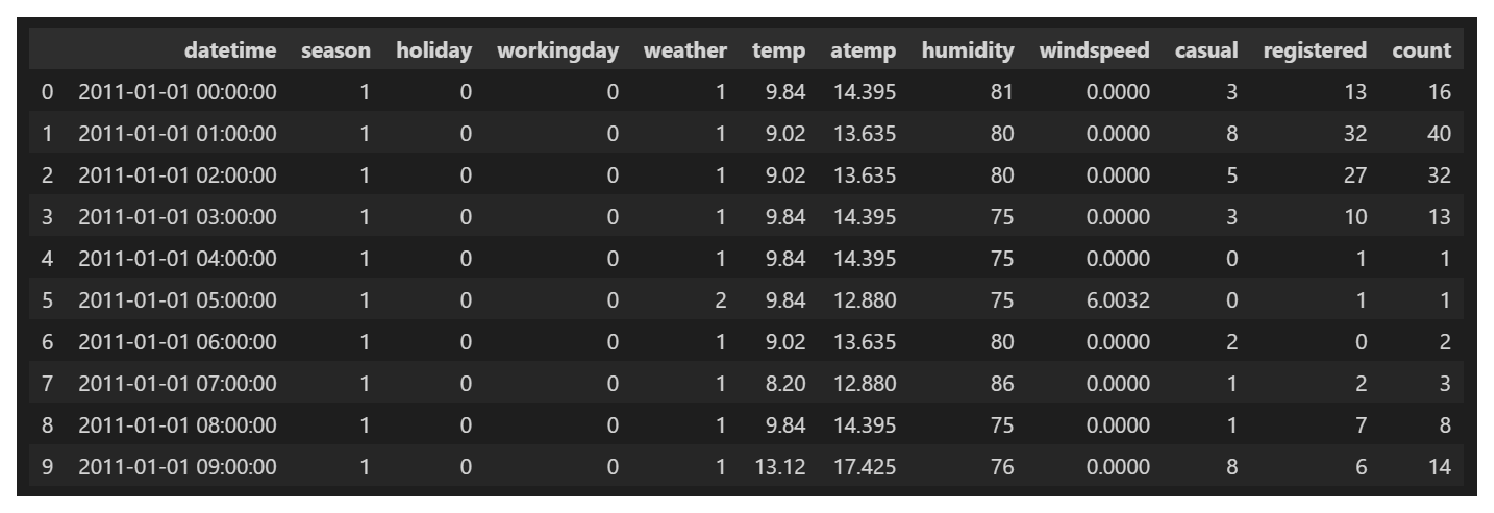
\includegraphics[width=0.9\textwidth]{figures/DataDescription.eps}\\
  \caption{Data Preview}\label{fig:dataPreview}
\end{figure}
\end{center}
\bigskip
\end{slide}

\begin{slide}[toc=,bm=]{Data Type}
\begin{center}
\begin{figure}
  \centering
  \selectcolormodel{rgb}
  %\missingfigure{Testing.}
  
\includegraphics[width=0.3\textwidth]{figures/DataType.eps}\\
  \caption{Data Type}\label{fig:dataType}
\end{figure}
\end{center}
\bigskip
\end{slide}



%%==========================================================================================
%%
\begin{slide}{Necessary Data Cleansing \& Transformation}
\begin{center}
    \begin{itemize}
    \item Check the skewness distribution to ensure the model’s ability (especially regression based models), which trains the model to deal less with rare cases on extreme values.
    \item Check any standardization need to be taken on the numeric data type
    \item Check any independent variables highly correlated
    \item Check any hypothesis can be made based on the raw data and any further transformation can be taken
    \end{itemize}
\end{center}
\bigskip
\end{slide}
%%
%%==========================================================================================

\begin{slide}[toc=,bm=]{Skewness Analysis}
\twocolumn{
\begin{figure}
  \centering
  \selectcolormodel{rgb}
  %\missingfigure{Testing.}
  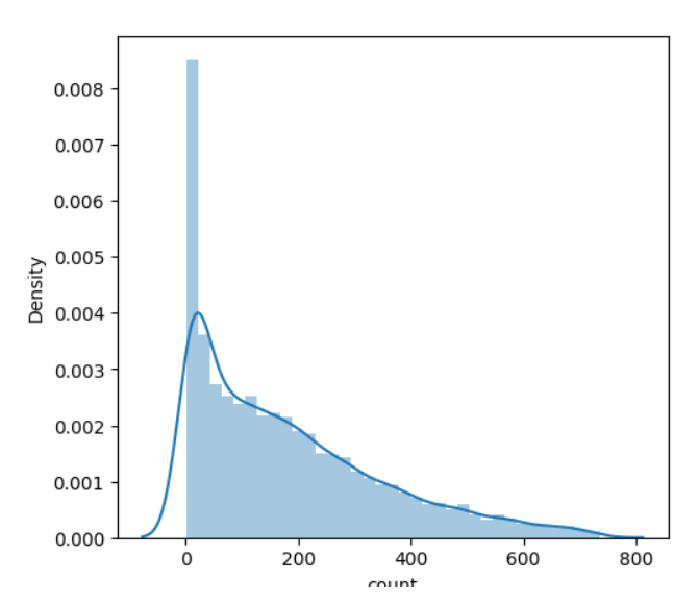
\includegraphics[width=0.6\textwidth]{figures/CountDistribution.eps}\\
  \caption{Count Distribution}\label{fig:CountDistribution}
\end{figure}
}{
\begin{figure}
  \centering
  \selectcolormodel{rgb}
  %\missingfigure{Testing.}
  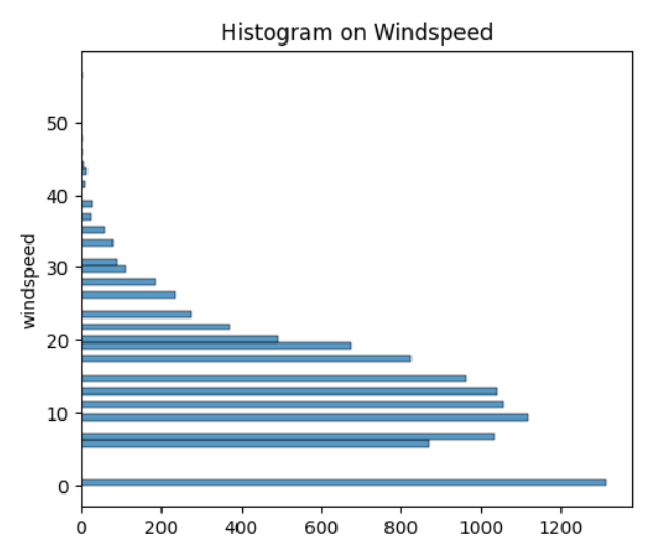
\includegraphics[width=0.6\textwidth]{figures/windspeed.eps}\\
  \caption{Windspeed}\label{fig:windspeed}
\end{figure}
}
\end{slide}
%%
%%==========================================================================================

\begin{slide}[toc=,bm=]{Outlier Analysis}
\begin{figure}
  \centering
  \selectcolormodel{rgb}
  %\missingfigure{Testing.}
  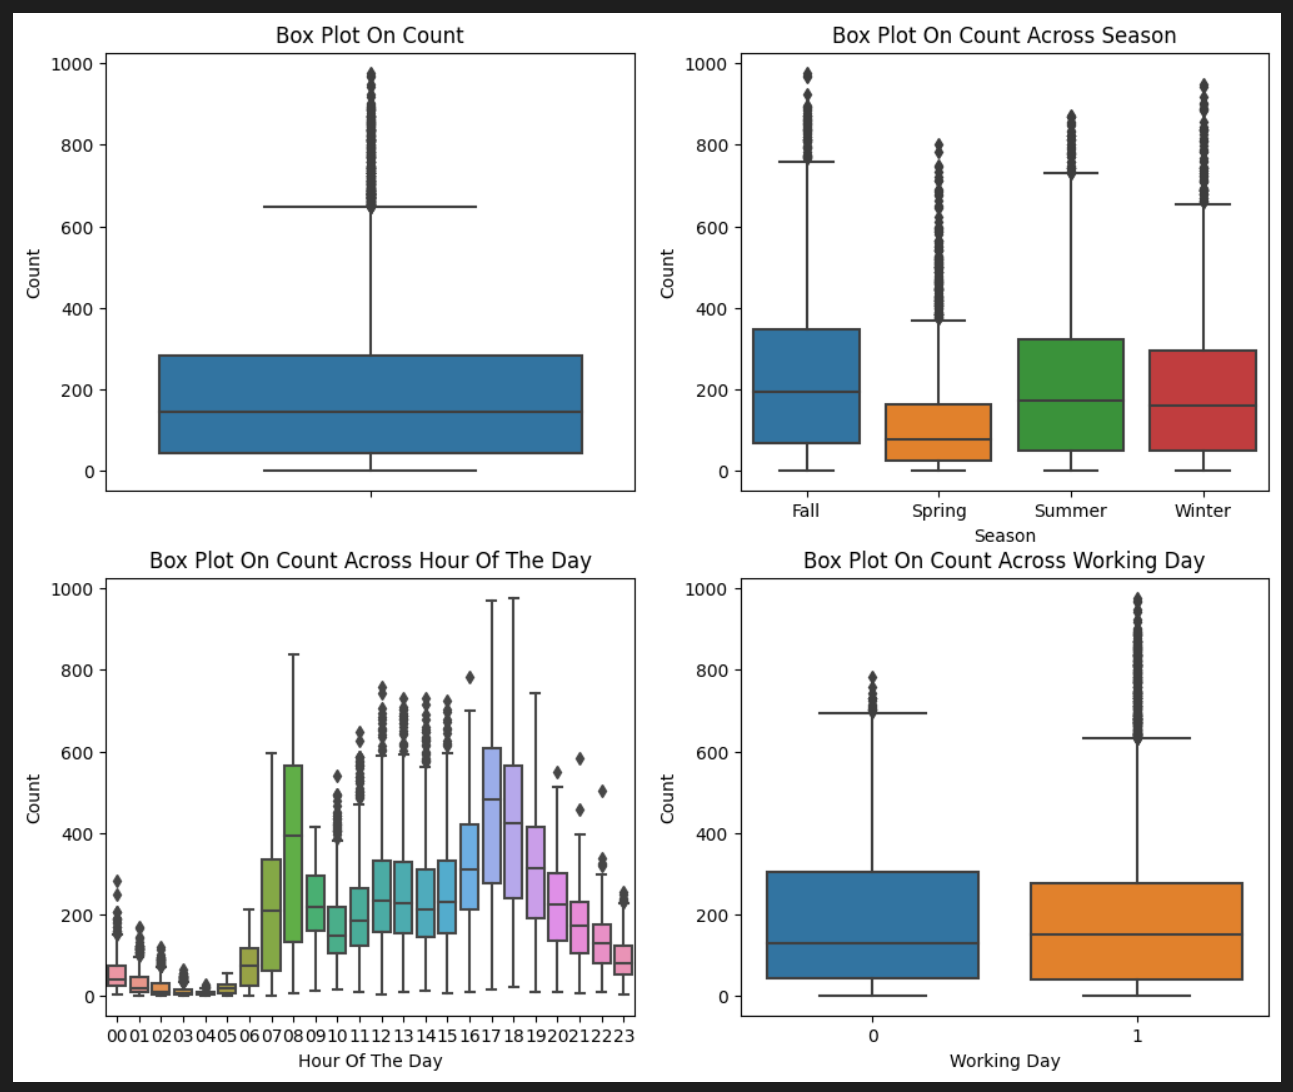
\includegraphics[width=0.6\textwidth]{figures/DataOutliers.eps}\\
  \caption{Data Outliers}\label{fig:DataOutliers}
\end{figure}
\end{slide}
%%
%%==========================================================================================

\begin{slide}[toc=,bm=]{Correlation Analysis}
\begin{figure}
  \centering
  \selectcolormodel{rgb}
  %\missingfigure{Testing.}
  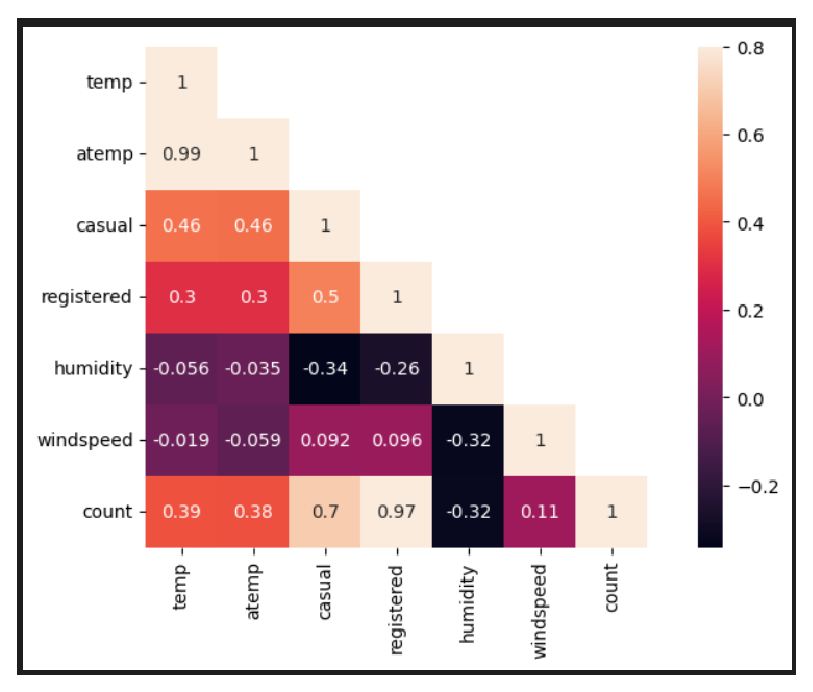
\includegraphics[width=0.6\textwidth]{figures/Correlation.eps}\\
  \caption{Correlation}\label{fig:Correlation}
\end{figure}
\end{slide}


\begin{slide}[toc=,bm=]{Insights Visualization - 1}
\begin{figure}
  \centering
  \selectcolormodel{rgb}
  %\missingfigure{Testing.}
  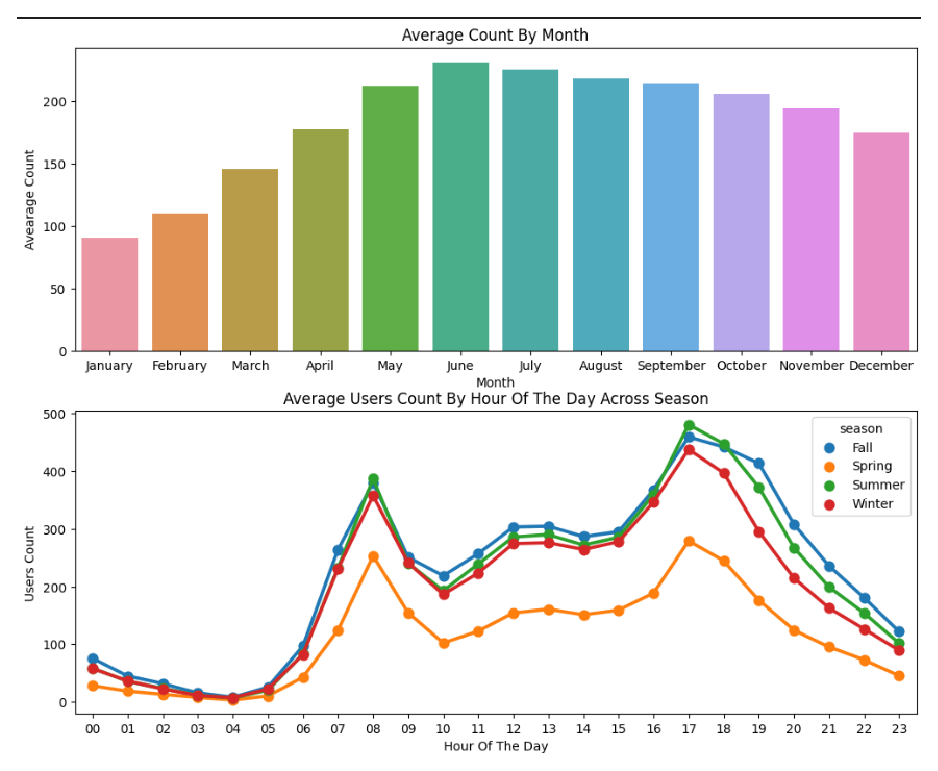
\includegraphics[width=0.6\textwidth]{figures/Vis-1.eps}\\
  \caption{Insights - 1}\label{fig:Insights1}
\end{figure}
\end{slide}

\begin{slide}[toc=,bm=]{Insights Visualization - 2}
\begin{figure}
  \centering
  \selectcolormodel{rgb}
  %\missingfigure{Testing.}
  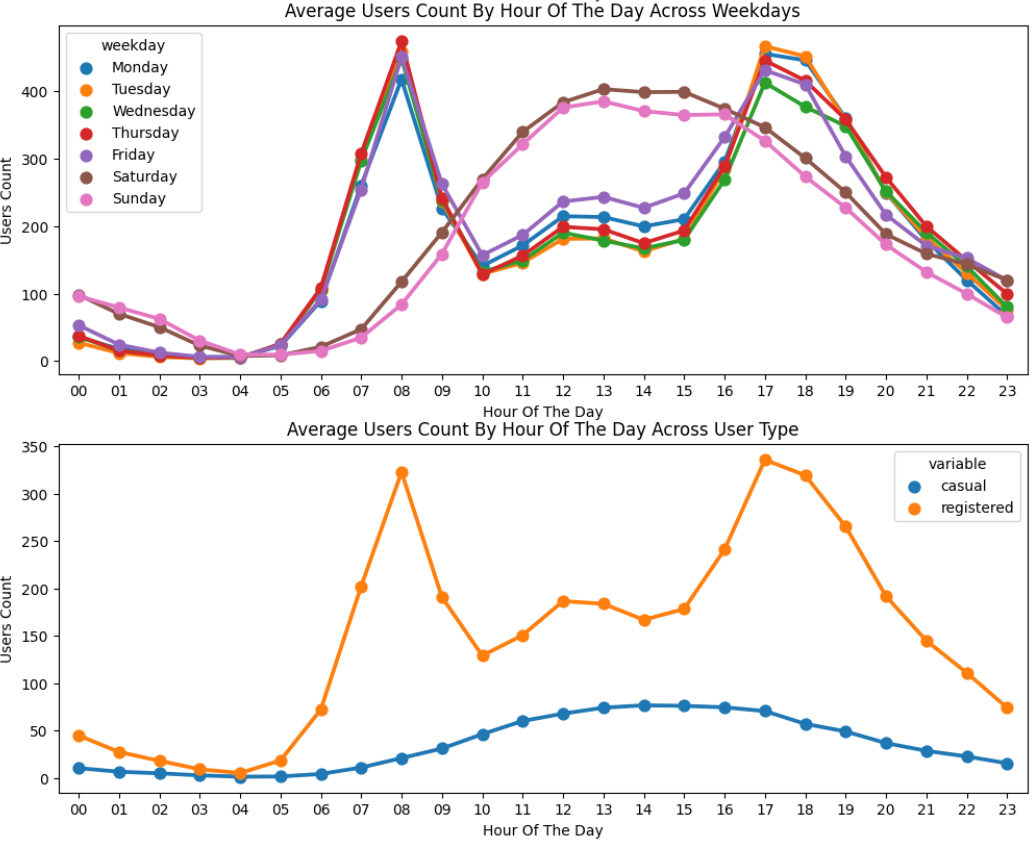
\includegraphics[width=0.6\textwidth]{figures/Vis-2.eps}\\
  \caption{Insights - 2}\label{fig:Insights2}
\end{figure}
\end{slide}
%%
%%==========================================================================================

\section{Model Selection}


%%==========================================================================================
%%
\begin{slide}{Linear Regression}
Linear regression - the linear regression fits a linear model with coefficients w = (w1, …, wp) to minimize the residual sum of squares between the observed targets in the dataset, and the targets predicted by the linear approximation. In this case, we can also apply the following two extra methods to increase the accuracy: 
    \begin{itemize}
    \item Use the grid search (GridSearchCV) to exhaustively search over specified parameter values for an estimation; 
    \item Use the regularization penalty (Ridge) to balance the model prediction by giving an l2-norm regularization.
    \end{itemize}
\end{slide}
%%
%%==========================================================================================
\begin{slide}{Ensemble}
Ensemble Models (averaging or boosting methods) 
    \begin{itemize}
    \item In averaging methods, the driving principle is to build several estimators independently and then to average their predictions. On average, the combined estimator is usually better than any of the single base estimator because its variance is reduced. 
    \item In boosting methods, base estimators are built sequentially and one tries to reduce the bias of the combined estimator. The motivation is to combine several weak models to produce a powerful ensemble.
    \end{itemize}
\end{slide}
%%
%%==========================================================================================

%%==========================================================================================
\section{Experiment \& Outcome}

%%==========================================================================================
%%
\begin{slide}{Experiment \& Outcome}
\begin{figure}
  \centering
  \selectcolormodel{rgb}
  %\missingfigure{Testing.}
  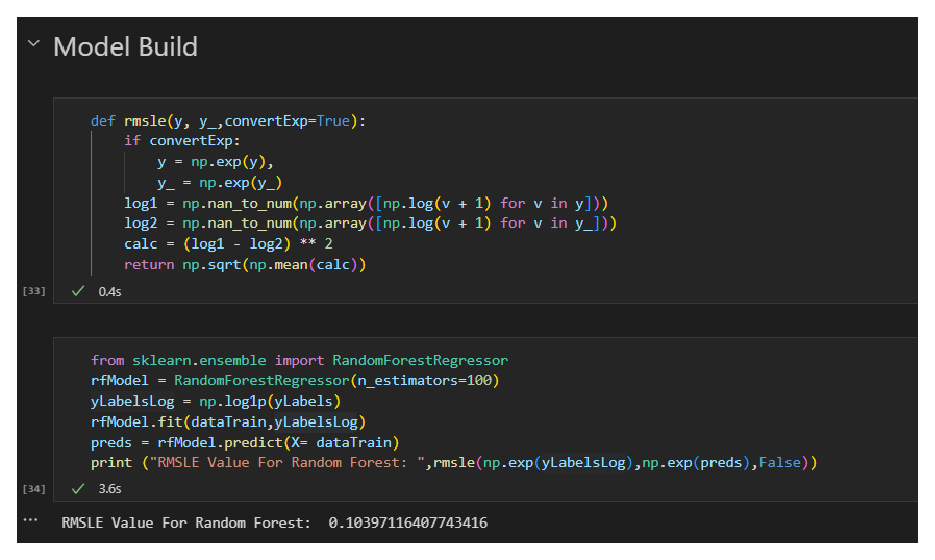
\includegraphics[width=0.9\textwidth]{figures/model.eps}\\
  \caption{Model}\label{fig:Model}
\end{figure}
\end{slide}

%%
%%==========================================================================================




%%==========================================================================================
% TODO: Contact Page
\begin{wideslide}[toc=,bm=]{Contact Information}
\centering
\vspace{\stretch{1}}
\twocolumn[
lcolwidth=0.35\linewidth,
rcolwidth=0.65\linewidth
]
{
% \centerline{
\includegraphics[scale=.2]{tulip-logo.eps}}
}
{
\vspace{\stretch{1}}
Qi Chu\\
School of Information Technology\\
Deakin University, Australia
\begin{description}
 \item[\textcolor{orange}{\faEnvelope}] \href{mailto:chuqi@deakin.edu.au}
 {\textsc{\footnotesize{chuqi@deakin.edu.au}}}

 \item[\textcolor{orange}{\faHome}] \href{http://www.tulip.org.au}
 {\textsc{\footnotesize{Team for Universal Learning and Intelligent Processing}}}
\end{description}
}
\vspace{\stretch{1}}
\end{wideslide}

\end{document}

\endinput
